\chapter{Water- en mineralenvoorziening van planten}\label{ch:b1:plant-water-minerals}

Een maïsplant onttrekt in juli een liter water per dag aan een bodem die
voor de hand droog aanvoelt, en daarmee de dertig milligram stikstof, als
nitraat, die zij nodig heeft om een dag groei op te bouwen. Zij heeft geen
pomp. Het water komt binnen omdat de \omterm{def:b1:flowering-plant-organization:organs}{wortel} droger is dan de bodem, in de
precieze zin van \cref{ch:b1:membranes-transport}; het nitraat komt binnen
omdat de wortelcellen er \omterm{def:b1:water-small-molecules:atp}{ATP} aan besteden; en beide moeten één enkele laag
\omterm{def:b1:cell-unit-of-life:cell}{cellen} passeren waarvan de wanden met was zijn afgedicht voordat zij het
\omterm{def:b1:flowering-plant-organization:tissues}{xyleem} bereiken. Dit hoofdstuk beschrijft de \omterm{def:b1:flowering-plant-organization:organs}{wortel} als opnemend \omterm{def:b1:mammal-organization:organ}{orgaan}, de
waterpotentialen die water van bodem naar \omterm{def:b1:flowering-plant-organization:tissues}{xyleem} drijven, de mineralen die
een plant nodig heeft en hoe zij die opneemt, het bijzondere geval van
stikstof, en de schimmels en bacteriën die de meeste \omterm{def:b1:flowering-plant-organization:organs}{wortels} inschakelen om
een deel van het werk te doen.

\section{De wortel als opnemend orgaan}

\begin{definition}[Apoplast, symplast en endodermis]\label{def:b1:plant-water-minerals:pathways}
\index{apoplast}\index{symplast}\index{band van Caspary}
Water en opgeloste stoffen doorkruisen de wortelschors langs twee wegen: de
\emph{apoplast}, het aaneengesloten stelsel van \omterm{prop:b1:carbohydrates:wall}{celwanden} en holten tussen
de \omterm{def:b1:cell-unit-of-life:cell}{cellen}, waardoor zij zich verplaatsen zonder enig membraan te passeren;
en de \emph{symplast}, het aaneengesloten \omterm{def:b1:cell-unit-of-life:cell}{cytoplasma} van de \omterm{def:b1:cell-unit-of-life:cell}{cellen} die door
plasmodesmata zijn verbonden (\cref{ch:b1:eukaryotic-cell}), dat wordt
betreden door één plasmamembraan te passeren. Aan de binnengrens van de
schors versperd de \emph{\omterm{prop:b1:flowering-plant-organization:stemroot}{endodermis}}
(\cref{ch:b1:flowering-plant-organization}) de apoplast: een band van
suberine en lignine, de \emph{band van Caspary}, doordrenkt haar radiale
wanden, zodat alles wat de centrale cilinder binnenkomt door het membraan
van een endodermiscel moet. De transporteiwitten van dat membraan bepalen
dus wat het \omterm{def:b1:flowering-plant-organization:tissues}{xyleem} bereikt, en verhinderen dat wat in het \omterm{def:b1:flowering-plant-organization:tissues}{xyleem} is geladen
weer weglekt.
\end{definition}

\begin{omfigure}
\begin{tikzpicture}[font=\footnotesize, >=Stealth, line cap=round]
  % row of cortex cells, endodermis, xylem
  \foreach \i in {0,1,2,3} {
    \draw[thick, omDef!60!black, fill=omDef!6] (1.6*\i,0) rectangle (1.6*\i+1.4,1.6);
    \draw[thick, omDef!60!black] (1.6*\i+0.15,0.15) rectangle (1.6*\i+1.25,1.45);
  }
  \node[anchor=south] at (2.9,1.7) {schorscellen (wand, dan membraan)};
  % endodermis cell with Casparian strip on radial walls
  \draw[thick, omDef!60!black, fill=omProp!12] (6.6,0) rectangle (8.0,1.6);
  \draw[thick, omDef!60!black] (6.75,0.15) rectangle (7.85,1.45);
  \draw[line width=4pt, omThm] (6.6,0.35) -- (6.6,1.25); \draw[line width=4pt, omThm] (8.0,0.35) -- (8.0,1.25);
  \node[anchor=south, align=center] at (7.3,1.7) {endodermis:\\ band van Caspary (rood)};
  % xylem
  \draw[thick, omDef!60!black, fill=omDef!25] (8.4,0) rectangle (9.8,1.6);
  \node at (9.1,0.8) {xyleem};
  % apoplast path: along walls, blocked at strip
  \draw[->, thick, omExo!70!black] (-0.6,0.08) -- (6.5,0.08);
  \draw[thick, omExo!70!black] (6.5,0.08) -- (6.5,0.3);
  \node[omExo!70!black, font=\scriptsize] at (6.2,-0.2) {versperd};
  \node[anchor=east, omExo!70!black, align=right, font=\scriptsize] at (-0.7,0.08) {apoplast:\\ door de wanden};
  % symplast path: through cells via plasmodesmata
  \draw[->, thick, omProp!80!black] (-0.6,0.8) -- (0.15,0.8);
  \foreach \i in {0,1,2,3} { \draw[->, thick, omProp!80!black] (1.6*\i+1.25,0.8) -- (1.6*\i+1.75,0.8); }
  \draw[->, thick, omProp!80!black] (7.85,0.8) -- (8.4,0.8);
  \node[anchor=east, omProp!80!black, align=right, font=\scriptsize] at (-0.7,0.8) {symplast:\\ door de cellen};
  % transfer from apoplast into symplast at endodermis
  \draw[->, thick, omThm] (6.4,0.25) -- (6.8,0.6);
  \node[anchor=north, align=center, gray] at (4.6,-0.5) {apoplast: geen membraan gepasseerd tot de endodermis,\\ waar water en ionen een cel binnen moeten;\\ symplast: één membraan bij het wortelhaar, dan plasmodesmata:\\ de cel kiest wat het xyleem binnengaat};
\end{tikzpicture}

{\small De twee wegen door de wortelschors. De apoplastische weg loopt door
de wanden tot de \omterm{def:b1:plant-water-minerals:pathways}{band van Caspary} haar stopt; de symplastische weg passeert
één membraan bij de epidermis en loopt dan van \omterm{def:b1:cell-unit-of-life:cell}{cel} naar \omterm{def:b1:cell-unit-of-life:cell}{cel}. Beide komen
samen bij de membranen van de \omterm{prop:b1:flowering-plant-organization:stemroot}{endodermis}.}
\end{omfigure}

\begin{proposition}[Worteldruk]\label{prop:b1:plant-water-minerals:rootpressure}
\index{worteldruk}\index{guttatie}
De \omterm{prop:b1:flowering-plant-organization:stemroot}{endodermis} en de \omterm{def:b1:cell-unit-of-life:cell}{cellen} daarbinnen pompen ionen het \omterm{def:b1:flowering-plant-organization:tissues}{xyleem} in, wat de
\omterm{def:b1:membranes-transport:osmosis}{waterpotentiaal} van het \omterm{def:b1:flowering-plant-organization:tissues}{xyleem} verlaagt en er osmotisch water uit de schors
in trekt; wanneer de spruit weinig verdampt ('s nachts, in vochtige lucht),
hoopt het water zich op en wordt het xyleemsap omhoog geduwd onder een
positieve \emph{\omterm{prop:b1:plant-water-minerals:rootpressure}{worteldruk}} van enkele tienden van een megapascal ---
genoeg om bij kleine planten druppels uit de bladtoppen te persen
(\emph{\omterm{prop:b1:plant-water-minerals:rootpressure}{guttatie}}) en om door lucht geblokkeerde \omterm{def:b1:flowering-plant-organization:tissues}{vaten} opnieuw te vullen,
maar niet genoeg om sap tot in de top van een boom te tillen. Overdag neemt
de zuigkracht van de transpiratie (\cref{ch:b1:plant-transport}) het over
en verdwijnt de \omterm{prop:b1:plant-water-minerals:rootpressure}{worteldruk}.
\end{proposition}
\begin{proof}[Bewijsmateriaal]
Een \omterm{def:b1:flowering-plant-organization:organs}{stengel} die vlak boven de grond wordt doorgesneden laat uren lang sap
uit zijn stomp lopen, en een manometer op die stomp meet een druk van
\qtyrange{0.1}{0.3}{MPa}; het uitgetreden sap is rijker aan ionen dan de
bodemoplossing, en de stroom stopt wanneer de \omterm{def:b1:flowering-plant-organization:organs}{wortels} worden gekoeld of
met een \omterm{def:b1:enzymes:inhibitors}{remmer} van de ademhaling worden vergiftigd: de stroom wordt door
actieve ionenlading gedreven, niet door enige waterpomp.
\end{proof}

\section{Water: van bodem naar xyleem}

\begin{proposition}[De ladder van waterpotentialen]\label{prop:b1:plant-water-minerals:ladder}
\index{waterpotentiaal}
Water beweegt van bodem naar \omterm{def:b1:flowering-plant-organization:tissues}{xyleem} omdat de \omterm{def:b1:membranes-transport:osmosis}{waterpotentiaal}
(\cref{ch:b1:membranes-transport}) bij elke stap daalt:
\begin{center}
\small
\begin{tabular}{lr}
\hline
compartiment & $\Psi$ (\unit{MPa}) \\
\hline
vochtige bodem & $-0.03$ tot $-0.3$ \\
bodem op het verwelkingspunt & $-1.5$ \\
\omterm{def:b1:cell-unit-of-life:cell}{cel} van de wortelschors & $-0.3$ tot $-0.6$ \\
\omterm{def:b1:flowering-plant-organization:tissues}{xyleem} van de \omterm{def:b1:flowering-plant-organization:organs}{wortel} & $-0.5$ tot $-0.8$ \\
bladcellen & $-1.0$ tot $-2.0$ \\
lucht bij \qty{50}{\%} relatieve vochtigheid & $-95$ \\
\hline
\end{tabular}
\end{center}
De potentiaal van de bodem wordt vooral bepaald door de spanning waarmee
haar poriën water vasthouden (capillariteit); die van de \omterm{def:b1:cell-unit-of-life:cell}{cellen} door hun
opgeloste stoffen en hun \omterm{def:b1:eukaryotic-cell:plantcell}{turgor}; die van het \omterm{def:b1:flowering-plant-organization:tissues}{xyleem} door de spanning van de
verdampende kolom; die van de lucht door haar vochtigheid,
$\Psi = (RT/V_w)\ln(\text{RV})$, wat zelfs in vochtige lucht enorm is. De
verreweg steilste stap is de laatste, van \omterm{def:b1:flowering-plant-organization:organs}{blad} naar lucht: daar wordt
vrijwel de hele drijvende kracht besteed, en daarom regelen planten haar
met huidmondjes.
\end{proposition}

\begin{omfigure}
\begin{tikzpicture}
\begin{axis}[
  ybar, bar width=14pt,
  width=0.86\linewidth, height=5.8cm,
  axis x line=bottom, axis y line=left,
  ymin=-2.2, ymax=0.2,
  ylabel={waterpotentiaal $\Psi$ (\unit{MPa})},
  ylabel style={font=\small},
  symbolic x coords={bodem, wortelschors, wortelxyleem, stengelxyleem, bladcel, bladluchtholte},
  xtick=data, x tick label style={font=\small, rotate=20, anchor=north east},
  enlarge x limits=0.12, ytick={0,-0.5,-1,-1.5,-2},
  nodes near coords, nodes near coords style={font=\scriptsize, anchor=north},
  point meta=rawy,
  clip=false,
]
\addplot[fill=omDef!45, draw=omDef] coordinates {(bodem,-0.2) (wortelschors,-0.4) (wortelxyleem,-0.6) (stengelxyleem,-0.9) (bladcel,-1.3) (bladluchtholte,-1.5)};
\node[font=\scriptsize, anchor=west, align=left, xshift=9pt] at (axis cs:bladluchtholte,-0.3) {(lucht: $-95$,\\ buiten beeld)};
\end{axis}
\end{tikzpicture}

{\small De \omterm{def:b1:membranes-transport:osmosis}{waterpotentiaal} langs de weg door een verdampende maïsplant op
een zomerdag. Elke stap ligt lager dan de vorige; de val naar de
buitenlucht, honderd keer groter dan alle andere samen, is niet getekend.}
\end{omfigure}

\begin{method}[Een profiel van waterpotentialen lezen]\label{met:b1:plant-water-minerals:profile}
\begin{enumerate}
  \item Zet de compartimenten op volgorde met hun $\Psi$; water stroomt
        alleen van hoger naar lager, dus de reeks moet langs de weg dalen,
        anders keert de stroom om.
  \item Splits de $\Psi$ van elke \omterm{def:b1:cell-unit-of-life:cell}{cel} in $\Psi_s$ (opgeloste stoffen,
        negatief) en $\Psi_p$ (\omterm{def:b1:eukaryotic-cell:plantcell}{turgor}, positief); een wortelcel bij
        $\Psi = -0.4$ met $\Psi_s = -0.9$ heeft $\Psi_p = +0.5$.
        Xyleemwater heeft $\Psi_s \approx 0$ en een negatieve $\Psi_p$:
        het staat onder spanning.
  \item De stroom over een stap is het verschil in $\Psi$ maal de
        hydraulische geleiding van de barrière; de \omterm{prop:b1:flowering-plant-organization:stemroot}{endodermis} en de
        huidmondjes zijn de twee stappen met een lage geleiding waar de
        plant regelt.
  \item Droogt de bodem uit, dan daalt haar $\Psi$; bereikt die de waarde
        van het \omterm{def:b1:flowering-plant-organization:organs}{blad}, dan stopt de stroom en verwelkt de plant; bereikt
        de $\Psi_p$ van de bladcellen nul, dan hangt het \omterm{def:b1:flowering-plant-organization:organs}{blad}. Herstel
        vraagt een verandering van de bodem, niet van de plant.
\end{enumerate}
\end{method}

\begin{example}[Een liter per dag]\label{ex:b1:plant-water-minerals:litre}
De fijne \omterm{def:b1:flowering-plant-organization:organs}{wortels} van een maïsplant bieden zo'n \qty{0.2}{m^2} oppervlak met
een hydraulische geleiding van ongeveer \qty{2e-7}{m.s^{-1}.MPa^{-1}};
tussen een bodem op \qty{-0.2}{MPa} en een wortelxyleem op \qty{-0.6}{MPa}
is de flux $2\times 10^{-7}\times 0.4\times 0.2 = \qty{1.6e-8}{m^3/s}$ ---
anderhalve liter per dag, die allemaal via de \omterm{def:b1:flowering-plant-organization:organs}{bladeren} verloren gaat. De
\omterm{def:b1:flowering-plant-organization:organs}{wortel} verricht er geen arbeid voor: de transpiratie van het \omterm{def:b1:flowering-plant-organization:organs}{blad} zet de
spanning, en de bodem levert het water zolang haar potentiaal boven die van
de \omterm{def:b1:flowering-plant-organization:organs}{wortel} blijft.
\end{example}

\section{Minerale voeding}

\begin{definition}[Essentiële elementen]\label{def:b1:plant-water-minerals:elements}
\index{essentieel element}\index{macronutriënt}\index{micronutriënt}
Een element is \emph{essentieel} voor een plant als de plant haar
levenscyclus er niet zonder kan voltooien en geen ander element het kan
vervangen. Het zijn er zeventien: koolstof, waterstof en zuurstof uit lucht
en water; de \emph{macronutriënten} die per kilogram droge massa in grammen
uit de bodem worden gehaald --- stikstof (als nitraat of ammonium), fosfor
(fosfaat), kalium, calcium, magnesium, zwavel (sulfaat); en de
\emph{micronutriënten} die in milligrammen of minder nodig zijn --- ijzer,
mangaan, zink, koper, boor, molybdeen, chloor, nikkel. Stikstof bouwt
\omterm{def:b1:proteins:peptide}{eiwitten} en nucleïnezuren; fosfor de \omterm{def:b1:nucleic-acids:nucleotide}{nucleotiden} en de membranen; kalium is
het belangrijkste kation van de \omterm{def:b1:cell-unit-of-life:cell}{cel} en het osmotisch middel van de
huidmondjes; magnesium zit in de \omterm{def:b1:photosynthesis:pigments}{chlorofyl}; ijzer in de cytochromen en in
ferredoxine; molybdeen in \omterm{prop:b1:plant-water-minerals:nitrate}{nitraatreductase} en nitrogenase.
\end{definition}

\begin{proposition}[Hoe de lijst is opgesteld]\label{prop:b1:plant-water-minerals:hydroponics}
De essentiële elementen zijn gevonden door planten te kweken in water dat
alleen bekende zouten bevatte.
\end{proposition}
\begin{proof}[Bewijsmateriaal]
Sachs en Knop (jaren 1860) kweekten planten tot volwassenheid op
oplossingen van enkele minerale zouten, geheel zonder bodem, en bewezen
daarmee dat de bodem niets anders levert dan mineralen en steun; door
telkens één zout weg te laten kreeg elk element een kenmerkende ziekte, die
genas zodra het weer werd toegevoegd. De \omterm{def:b1:plant-water-minerals:elements}{micronutriënten} werden later
gevonden, naarmate scheikundigen de zouten zuiverder kregen: een plant die
molybdeen mist, nodig in een deel op tien miljoen, reduceert geen nitraat.
De techniek, hydrocultuur, voedt nu kassen.
\end{proof}

\begin{omfigure}
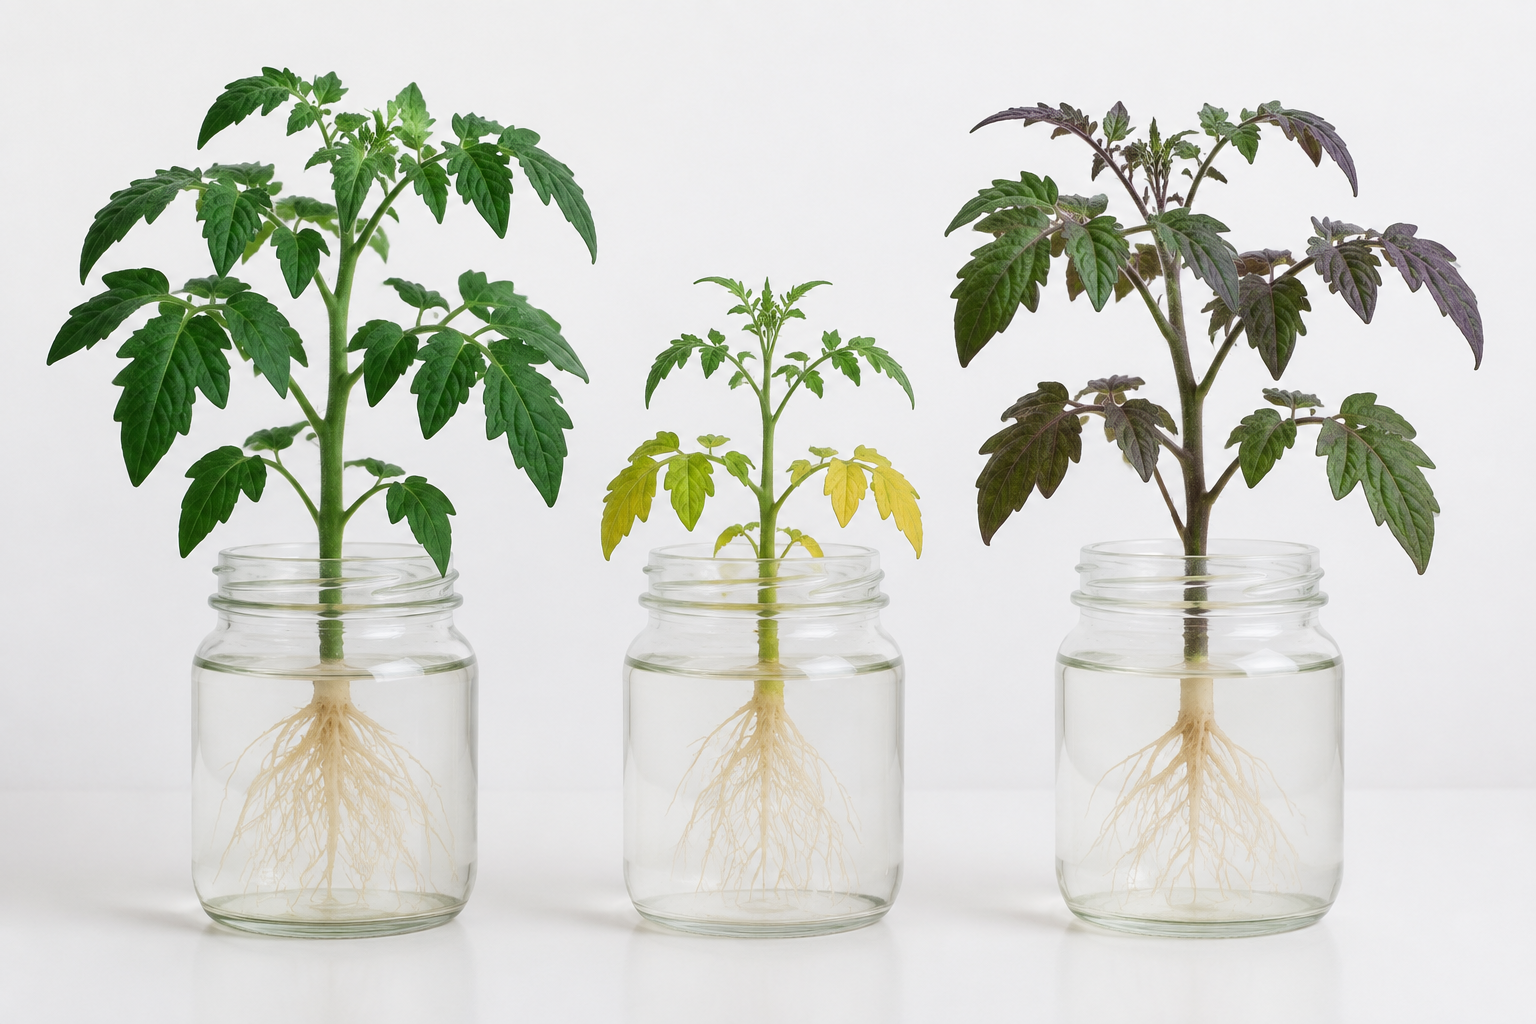
\includegraphics[width=0.6\linewidth]{images/book3/ai/b3-23-nutrient-deficiency.png}

{\small Drie tomatenplanten in voedingsoplossingen: volledig (links),
zonder stikstof (midden: achtergebleven, met vergelende oude \omterm{def:b1:flowering-plant-organization:organs}{bladeren}
waarvan de stikstof naar de jonge wordt verplaatst), zonder fosfor (rechts:
donkere \omterm{def:b1:flowering-plant-organization:organs}{bladeren} met een paarse zweem). Elk ontbrekend element heeft zijn
eigen handtekening.}
\end{omfigure}

\begin{method}[Een gebrek lezen]\label{met:b1:plant-water-minerals:deficiency}
\begin{enumerate}
  \item Vraag waar het verschijnsel optreedt. Elementen die de plant in
        het floëem kan verplaatsen (N, P, K, Mg) worden aan oude \omterm{def:b1:flowering-plant-organization:organs}{bladeren}
        onttrokken om de jonge te voeden: de oude \omterm{def:b1:flowering-plant-organization:organs}{bladeren} tonen het
        gebrek eerst. Elementen die zij niet kan verplaatsen (Ca, Fe, B)
        blijven achter waar zij zijn neergelegd: de jonge \omterm{def:b1:flowering-plant-organization:organs}{bladeren} en de
        groeitoppen tonen het.
  \item Vraag wat het element doet: geen stikstof, weinig \omterm{def:b1:photosynthesis:pigments}{chlorofyl} en
        \omterm{def:b1:proteins:peptide}{eiwit} --- bleek en achtergebleven; geen magnesium of ijzer, dan
        faalt de \omterm{def:b1:photosynthesis:pigments}{chlorofyl} --- gele \omterm{def:b1:flowering-plant-organization:organs}{bladeren} met groene nerven; geen
        kalium, dan verschroeien de bladranden; geen calcium, dan sterven
        de groeitoppen.
  \item Bevestig het door alleen het verdachte element toe te dienen en
        de nieuwe groei te bekijken.
\end{enumerate}
\end{method}

\begin{proposition}[Actieve opname van ionen]\label{prop:b1:plant-water-minerals:uptake}
\index{protonpomp}
De bodemoplossing bevat ionen in micromollen tot enkele millimollen per
liter; de wortelcellen houden kalium op \qty{100}{mmol/L}, fosfaat op
\qty{10}{}, nitraat op enkele. De opname gaat dus meestal bergopwaarts en
wordt met \omterm{def:b1:water-small-molecules:atp}{ATP} betaald, maar indirect: een \emph{\omterm{prop:b1:plant-water-minerals:uptake}{protonpomp}} in het
plasmamembraan (\cref{ch:b1:membranes-transport}) voert
$\mathrm{H^+}$ uit, waardoor de buitenkant \omterm{def:b1:water-small-molecules:ph}{zuur} wordt en de binnenkant
\qtyrange{-120}{-200}{mV} negatief; kationen als $\mathrm{K^+}$ komen dan
door \omterm{def:b1:membranes-transport:transporters}{kanalen} langs de elektrische gradiënt binnen, en anionen
($\mathrm{NO_3^-}$, $\mathrm{H_2PO_4^-}$, $\mathrm{SO_4^{2-}}$) via
\omterm{prop:b1:membranes-transport:secondary}{symporters} die op de terugkerende protonen meeliften. De transporteiwitten
zijn selectief: kalium wordt honderd keer gemakkelijker opgenomen dan
natrium van dezelfde lading en vrijwel dezelfde grootte, en de plant houdt
natrium zelfs in zoute bodem buiten. \omterm{def:b1:flowering-plant-organization:organs}{Wortels} besteden een derde van de
ademhaling van de plant aan dit transport.
\end{proposition}

\section{Stikstof}

\begin{proposition}[Van nitraat tot aminozuur]\label{prop:b1:plant-water-minerals:nitrate}
\index{nitraatreductase}\index{stikstofassimilatie}
De meeste planten nemen stikstof op als nitraat. In het \omterm{def:b1:eukaryotic-cell:organelle}{cytosol} reduceert
\emph{\omterm{prop:b1:plant-water-minerals:nitrate}{nitraatreductase}}, een molybdeenenzym, het tot nitriet met elektronen
van NADH; in de \omterm{def:b1:eukaryotic-cell:plastid}{plastide} reduceert \emph{\omterm{prop:b1:plant-water-minerals:nitrate}{nitrietreductase}} het nitriet tot
ammonium met elektronen van ferredoxine; en ammonium wordt onmiddellijk
vastgelegd in glutamine en \omterm{def:b1:biosyntheses-integration:nitrogen}{glutamaat}
(\cref{ch:b1:biosyntheses-integration}) --- ammonium zelf is giftig en hoopt
zich nooit op. De hele reductie kost acht elektronen per stikstofatoom, een
tiende van de fotosynthetische elektronenstroom van een \omterm{def:b1:flowering-plant-organization:organs}{blad} op een
nitraatrijke bodem, en een \omterm{def:b1:flowering-plant-organization:organs}{blad} doet er veel van in het licht, rechtstreeks
uit de ferredoxine van de chloroplast. Ammonium wordt, waar de bodem het
biedt, rechtstreeks opgenomen en slaat die kosten over.
\end{proposition}

\begin{definition}[Stikstofbinding en wortelknolletjes]\label{def:b1:plant-water-minerals:nodules}
\index{stikstofbinding}\index{wortelknolletje}\index{Rhizobium}
Geen enkele eukaryoot kan de $\mathrm{N_2}$ van de lucht gebruiken.
Sommige bacteriën wel: \emph{nitrogenase} verbreekt de drievoudige binding
van $\mathrm{N_2}$ en reduceert die tot twee ammoniak, tegen zestien \omterm{def:b1:water-small-molecules:atp}{ATP} en
acht elektronen per molecuul, en alleen waar zuurstof is uitgesloten.
Vlinderbloemigen (erwten, bonen, klaver) huisvesten zulke bacteriën
(\emph{Rhizobium}) in \emph{wortelknolletjes}: de plant bouwt een kamer,
voedt de bacteriën met suiker, en houdt de zuurstof laag met een rood
\omterm{def:b1:proteins:peptide}{eiwit}, leghemoglobine, dat haar aan de ademhaling van de bacteriën aflevert
bij een concentratie die te laag is om het \omterm{def:b1:enzymes:enzyme}{enzym} te schaden; de bacteriën
geven ammonium terug, dat de plant tot \omterm{def:b1:proteins:aminoacid}{aminozuren} omzet. Een klaverveld
bindt honderd kilogram stikstof per hectare per jaar, waarvoor de plant een
tiende van haar fotosynthese betaalt. De stikstofkringloop als geheel hoort
in het deel van jaar 2.
\end{definition}

\begin{omfigure}
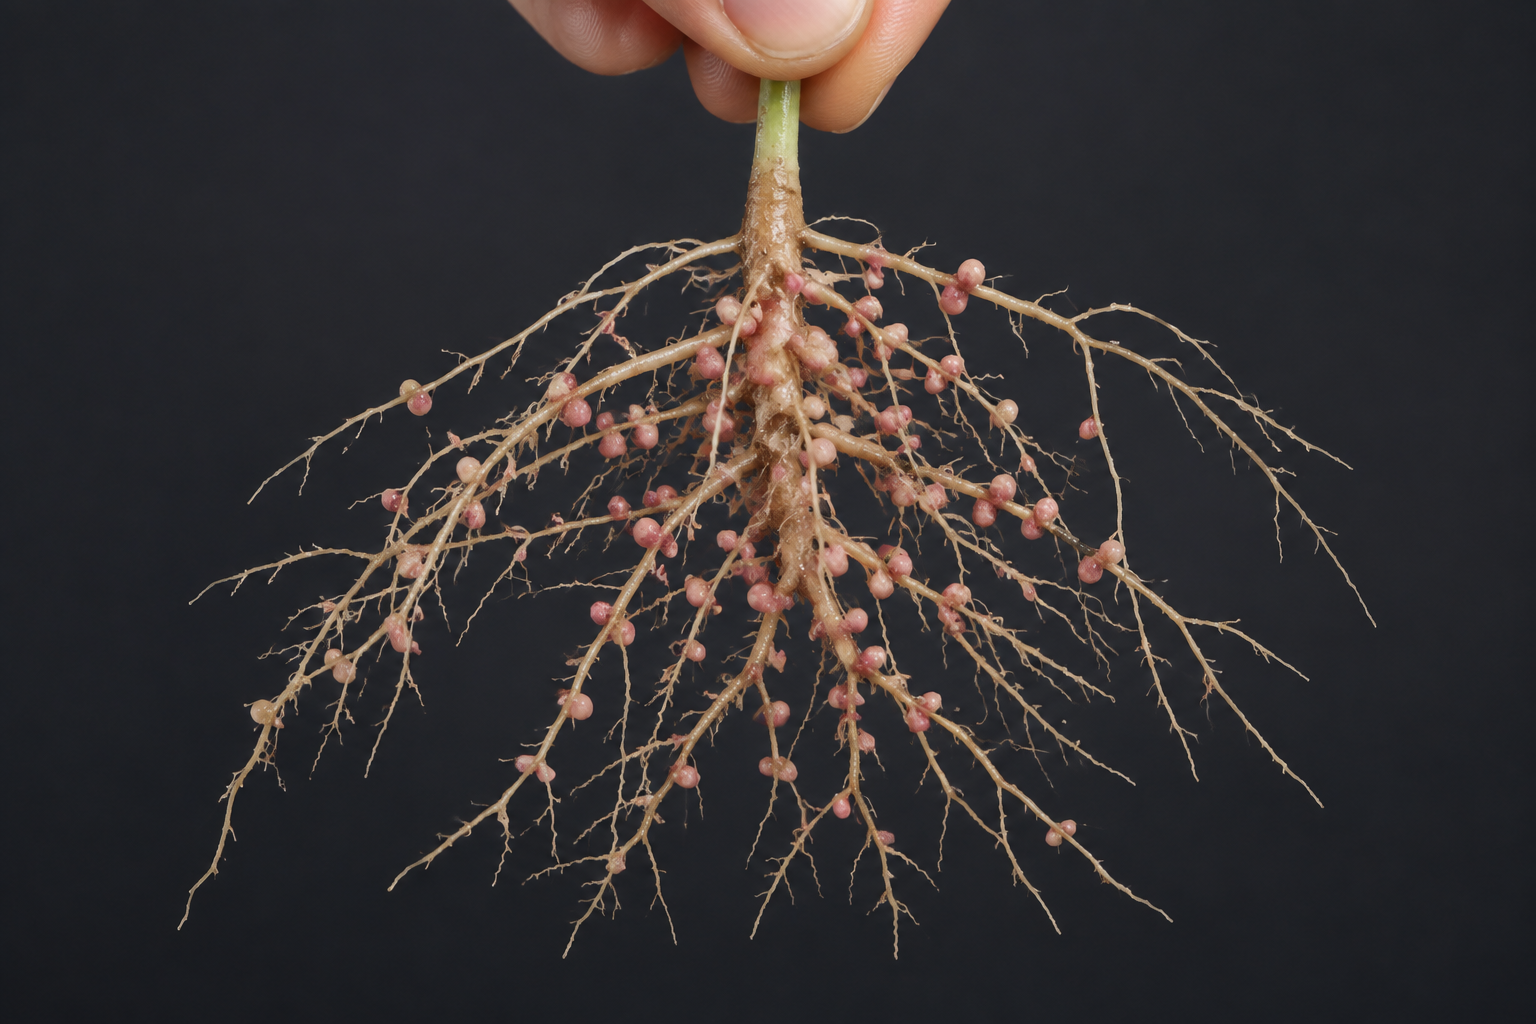
\includegraphics[width=0.52\linewidth]{images/book3/ai/b3-23-root-nodules.png}

{\small Knolletjes aan de \omterm{def:b1:flowering-plant-organization:organs}{wortels} van een vlinderbloemige: elk is een kamer
van plantenweefsel gevuld met bacteriën, roze van het leghemoglobine, waar
stikstof uit de lucht wordt gebonden.}
\end{omfigure}

\begin{example}[De prijs van stikstof]\label{ex:b1:plant-water-minerals:priceN}
Een maïsplant heeft ongeveer \qty{30}{mg} stikstof per dag nodig; uit
nitraat op \qty{2}{mmol/L} haalt zij dat uit de liter water die zij
verdampt, en zij besteedt enkele honderden millimollen elektronen aan de
reductie ervan. Een klaverplant die dezelfde hoeveelheid bindt betaalt
\qty{16}{} \omterm{def:b1:water-small-molecules:atp}{ATP} per $\mathrm{N_2}$ plus het reductiemiddel --- ruwweg
\qty{6}{g} suiker per gram stikstof, zo'n \qty{0.2}{g} per dag, een tiende
van haar productie --- en kan groeien op een bodem zonder enig nitraat.
Boeren wisselen al tweeduizend jaar vlinderbloemigen met granen af om die
stikstof van de ene akker naar de volgende te brengen.
\end{example}

\section{Partners in de bodem}

\begin{definition}[Mycorrhiza]\label{def:b1:plant-water-minerals:mycorrhiza}
\index{mycorrhiza}
Een \emph{mycorrhiza} is een verbond tussen een \omterm{def:b1:flowering-plant-organization:organs}{wortel} en een schimmel, dat
bij negen van de tien planten voorkomt. In de gewoonste vorm groeien de
hyfen van de schimmel de schorscellen in en vertakken zich daarbinnen tot
\emph{arbusculen}, het \omterm{prop:b1:organism-environment:surfaces}{uitwisselingsoppervlak}, terwijl buiten de \omterm{def:b1:flowering-plant-organization:organs}{wortel} een
net van hyfen van enkele micrometers dik de bodem meters ver verkent. De
schimmel levert fosfaat en andere weinig beweeglijke ionen, en water, die
de \omterm{def:b1:flowering-plant-organization:organs}{wortelharen} zelf niet konden bereiken; de plant levert suiker, een
tiende of meer van haar fotosynthese. Bomen van gematigde bossen dragen een
tweede vorm, waarbij de schimmel de worteltoppen omhult en zich tussen de
\omterm{def:b1:cell-unit-of-life:cell}{cellen} door vlecht; haar vruchtlichamen zijn de paddenstoelen van de
bosbodem.
\end{definition}
\begin{proof}[Bewijsmateriaal]
Zaailingen die op gesteriliseerde bodem worden gekweekt groeien slecht en
nemen weinig fosfaat op; geënt met sporen van de schimmel worden zij
enkele malen groter. Radioactief fosfaat dat buiten het bereik van de
\omterm{def:b1:flowering-plant-organization:organs}{wortels} in de bodem wordt gelegd verschijnt alleen in de plant als hyfen de
twee verbinden, en gemerkte koolstof die aan de \omterm{def:b1:flowering-plant-organization:organs}{bladeren} wordt gevoerd
verschijnt binnen een dag in de hyfen. Het doorsnijden van de hyfen met een
fijn gaas dat opgeloste stoffen maar geen schimmels doorlaat heft de winst
op.
\end{proof}

\begin{omfigure}
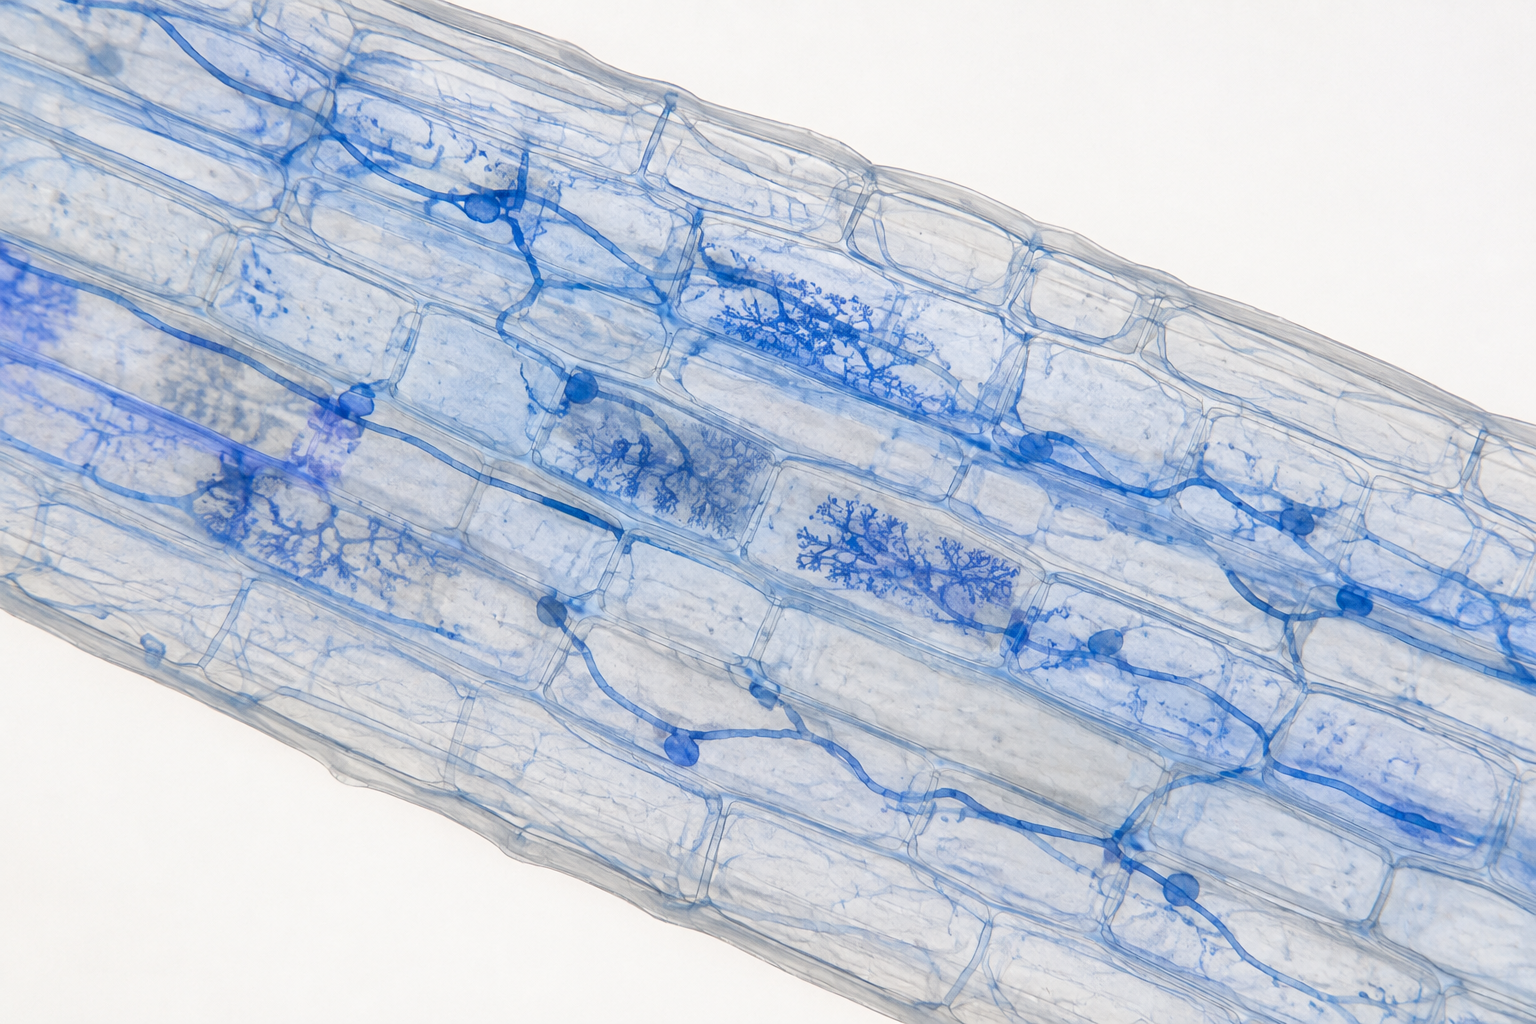
\includegraphics[width=0.52\linewidth]{images/book3/ai/b3-23-mycorrhiza.png}

{\small Een \omterm{def:b1:flowering-plant-organization:organs}{wortel} gekleurd om zijn mycorrhizaschimmel te tonen: hyfen die
tussen de \omterm{def:b1:cell-unit-of-life:cell}{cellen} lopen en zich daarbinnen tot arbusculen vertakken --- een
tweede opnemend oppervlak, door de plant van suiker voorzien.}
\end{omfigure}

\begin{example}[Waarom fosfaat een schimmel nodig heeft]\label{ex:b1:plant-water-minerals:phosphate}
Fosfaat hecht zich aan bodemdeeltjes en diffundeert een millimeter per dag;
een \omterm{def:b1:flowering-plant-organization:organs}{wortelhaar} neemt binnen enkele uren al het fosfaat op dat het kan
bereiken en wacht dan. Hyfen die tien keer dunner zijn dan een \omterm{def:b1:flowering-plant-organization:organs}{wortelhaar}
reiken per gram \omterm{def:b1:body-plans-tissues:tissue}{weefsel} tien keer verder, en een meter hyfe kost de plant
een duizendste van wat een meter \omterm{def:b1:flowering-plant-organization:organs}{wortel} kost. Voor nitraat, dat vrij met
het bodemwater meebeweegt, volstaan de eigen \omterm{def:b1:flowering-plant-organization:organs}{wortelharen}, en planten op
nitraatrijke bodems bouwen hun schimmel af; voor fosfaat is de schimmel het
verlengstuk van de \omterm{def:b1:flowering-plant-organization:organs}{wortel}.
\end{example}

\section{Opgaven}

\begin{exercise}[$\star$]\label{exo:b1:plant-water-minerals:1}
Omschrijf \omterm{def:b1:plant-water-minerals:pathways}{apoplast} en \omterm{def:b1:plant-water-minerals:pathways}{symplast}, en zeg wat de \omterm{def:b1:plant-water-minerals:pathways}{band van Caspary} doet.
\end{exercise}

\begin{exercise}[$\star$]\label{exo:b1:plant-water-minerals:2}
Noem de zes \omterm{def:b1:plant-water-minerals:elements}{macronutriënten} die een plant uit de bodem haalt en van elk één
rol.
\end{exercise}

\begin{exercise}[$\star$]\label{exo:b1:plant-water-minerals:3}
Lees uit de figuur van de waterpotentialen de $\Psi$ af in de bodem, het
wortelxyleem en de bladcel, en geef bij elke stap de stroomrichting.
\end{exercise}

\begin{exercise}[$\star$]\label{exo:b1:plant-water-minerals:4}
Waarom worden een stikstofgebrek en een ijzergebrek op verschillende
\omterm{def:b1:flowering-plant-organization:organs}{bladeren} zichtbaar?
\end{exercise}

\begin{exercise}[$\star\star$]\label{exo:b1:plant-water-minerals:5}
Een \omterm{def:b1:cell-unit-of-life:cell}{cel} van de wortelschors heeft $\Psi_s = \qty{-0.9}{MPa}$ en $\Psi_p =
\qty{0.5}{MPa}$; de bodem staat op \qty{-0.2}{MPa}, het \omterm{def:b1:flowering-plant-organization:tissues}{xyleem} op
\qty{-0.6}{MPa}. Toon aan dat water van bodem naar \omterm{def:b1:cell-unit-of-life:cell}{cel} naar \omterm{def:b1:flowering-plant-organization:tissues}{xyleem} stroomt,
en bereken de $\Psi_p$ van de \omterm{def:b1:cell-unit-of-life:cell}{cel} waarbij zij uit deze bodem geen water
meer zou opnemen.
\end{exercise}

\begin{exercise}[$\star\star$]\label{exo:b1:plant-water-minerals:6}
Bereken de \omterm{def:b1:membranes-transport:osmosis}{waterpotentiaal} van lucht bij \qty{90}{\%}, \qty{50}{\%} en
\qty{10}{\%} relatieve vochtigheid bij \qty{25}{\celsius} ($RT/V_w =
\qty{137}{MPa}$). Vergelijk met de bodem op het verwelkingspunt en
becommentarieer dat.
\end{exercise}

\begin{exercise}[$\star\star$]\label{exo:b1:plant-water-minerals:7}
Een wortelcel op \qty{-150}{mV} neemt $\mathrm{K^+}$ op van
\qty{0.1}{mmol/L} tot \qty{100}{mmol/L}. Bereken de nernstpotentiaal voor
deze verhouding bij \qty{25}{\celsius} en zeg of \omterm{def:b1:membranes-transport:transporters}{kanalen} alleen dat kunnen.
Herhaal dat voor nitraat bij \qty{0.5}{} buiten en \qty{5}{mmol/L} binnen.
\end{exercise}

\begin{exercise}[$\star\star$]\label{exo:b1:plant-water-minerals:8}
Leg uit waarom \omterm{prop:b1:plant-water-minerals:rootpressure}{guttatie} bij dageraad op gras te zien is maar nooit op een
hoge boom, en wat er met de \omterm{prop:b1:plant-water-minerals:rootpressure}{worteldruk} gebeurt zodra de transpiratie begint.
\end{exercise}

\begin{exercise}[$\star\star$]\label{exo:b1:plant-water-minerals:9}
Een plant wordt overgezet in een oplossing zonder molybdeen. Voorspel haar
groei op nitraat en op ammonium, en verklaar het verschil.
\end{exercise}

\begin{exercise}[$\star\star\star$]\label{exo:b1:plant-water-minerals:10}
Bereken de elektronen die per dag nodig zijn om \qty{30}{mg}
nitraatstikstof tot ammonium te reduceren, en het aantal NADPH-equivalenten;
vergelijk dat met de elektronen die een maïsblad van \qty{500}{cm^2} per
dag door zijn \omterm{def:b1:photosynthesis:zscheme}{fotosystemen} beweegt bij \qty{4}{\micro mol}
$\mathrm{CO_2}$ per vierkante meter per seconde (4 elektronen per
$\mathrm{CO_2}$, \qty{12}{h}).
\end{exercise}

\begin{exercise}[$\star\star\star$]\label{exo:b1:plant-water-minerals:11}
Een klaver bindt \qty{30}{mg} stikstof per dag bij \qty{16}{} \omterm{def:b1:water-small-molecules:atp}{ATP} en
\qty{8}{} elektronen per $\mathrm{N_2}$, en \qty{6}{g} suiker per gram
stikstof in totaal. Bereken de \omterm{def:b1:water-small-molecules:atp}{ATP} die nitrogenase alleen al besteedt, de
suiker die dat zou kosten (30 \omterm{def:b1:water-small-molecules:atp}{ATP} per glucose), en welk deel van de
\qty{6}{g} dat is. Waar gaat de rest heen?
\end{exercise}

\begin{exercise}[$\star\star\star$]\label{exo:b1:plant-water-minerals:12}
``Een \omterm{def:b1:flowering-plant-organization:organs}{wortel} is een mijnbouwbedrijf dat aannemers inhuurt.'' Bespreek dat in
een alinea: wat de \omterm{def:b1:flowering-plant-organization:organs}{wortel} zelf doet (water, beweeglijke ionen), wat hij
uitbesteedt (fosfaat, gebonden stikstof), wat hij betaalt, en wanneer hij
stopt met betalen.
\end{exercise}

\section{Vraagstuk: de waterpotentiaalladder van een maïswortel}

\begin{problem}[{Weekendvraagstuk --- water en nitraat uit een julibodem
een maïsplant in: de potentialen bij elke stap, de flux door de wortels, de
stikstof die zij aanvoert en de kosten van de reductie ervan, eindigend op
de dagelijkse waterflux de wortel in}]
\label{pb:b1:plant-water-minerals:1}
Een maïsplant in juli: oppervlak van de fijne \omterm{def:b1:flowering-plant-organization:organs}{wortels} \qty{0.2}{m^2},
hydraulische geleiding van de \omterm{def:b1:flowering-plant-organization:organs}{wortel} \qty{2e-7}{m.s^{-1}.MPa^{-1}};
bladoppervlak \qty{0.5}{m^2}. \omterm{def:b1:membranes-transport:osmosis}{Waterpotentiaal} van de bodem
\qty{-0.2}{MPa}; \omterm{def:b1:cell-unit-of-life:cell}{cellen} van de wortelschors met $\Psi_s = \qty{-0.9}{MPa}$
en $\Psi_p = \qty{0.5}{MPa}$; wortelxyleem \qty{-0.6}{MPa}; bladcellen
\qty{-1.3}{MPa}; lucht bij \qty{50}{\%} relatieve vochtigheid
($RT/V_w = \qty{137}{MPa}$). Nitraat in de bodem \qty{2}{mmol/L}; de plant
heeft \qty{30}{mg} stikstof per dag nodig. De reductie van nitraat tot
ammonium gebruikt 8 elektronen per stikstofatoom; de fotosynthese beweegt 4
elektronen per $\mathrm{CO_2}$ en het \omterm{def:b1:flowering-plant-organization:organs}{blad} legt \qty{4}{\micro mol}
$\mathrm{CO_2}$ per vierkante meter per seconde vast gedurende
\qty{12}{h}.

\medskip
\noindent\textbf{Deel I --- De ladder.}
\begin{enumerate}
  \item Bereken de \omterm{def:b1:membranes-transport:osmosis}{waterpotentiaal} van de \omterm{def:b1:cell-unit-of-life:cell}{cellen} van de wortelschors.
  \item Schrijf de reeks bodem, schors, \omterm{def:b1:flowering-plant-organization:tissues}{xyleem}, \omterm{def:b1:flowering-plant-organization:organs}{blad} op en controleer dat
        het water bij elke stap naar binnen en naar boven stroomt.
  \item Bereken de \omterm{def:b1:membranes-transport:osmosis}{waterpotentiaal} van de lucht.
  \item Bereken de val van bodem naar \omterm{def:b1:flowering-plant-organization:organs}{blad} en de val van \omterm{def:b1:flowering-plant-organization:organs}{blad} naar lucht;
        welk deel van het geheel is de laatste stap?
  \item De bodem droogt uit tot \qty{-0.9}{MPa}. Wat gebeurt er met de
        stroom naar de schorscellen, en met hun \omterm{def:b1:eukaryotic-cell:plantcell}{turgor}?
  \item De bodem droogt uit tot \qty{-1.5}{MPa}. Wat gebeurt er met de
        \omterm{def:b1:flowering-plant-organization:organs}{bladeren}, en waarom herstelt water geven hen?
\end{enumerate}

\medskip
\noindent\textbf{Deel II --- De flux.}
\begin{enumerate}[resume]
  \item Bereken de waterflux de \omterm{def:b1:flowering-plant-organization:organs}{wortels} in (geleiding $\times$
        oppervlak $\times$ het verschil tussen bodem en wortelxyleem).
  \item Zet die om in liters per dag.
  \item Alles gaat door transpiratie verloren. Bereken de transpiratie per
        vierkante meter \omterm{def:b1:flowering-plant-organization:organs}{blad} per uur, in grammen.
  \item Druk de transpiratie per vierkante meter \omterm{def:b1:flowering-plant-organization:organs}{blad} per seconde uit in
        millimol water (\qty{18}{g/mol}).
  \item De huidmondjes sluiten zich midden op de dag en de $\Psi$ van het
        \omterm{def:b1:flowering-plant-organization:organs}{blad} stijgt tot \qty{-0.9}{MPa} terwijl die van het \omterm{def:b1:flowering-plant-organization:tissues}{xyleem} tot
        \qty{-0.4}{MPa} stijgt. Bereken de flux opnieuw. Wat heeft de
        plant gedaan, en waarom?
  \item Waarom neemt de \omterm{def:b1:flowering-plant-organization:organs}{wortel} water op zonder energie te besteden,
        terwijl hij voor de opname van nitraat energie moet besteden?
\end{enumerate}

\medskip
\noindent\textbf{Deel III --- Stikstof.}
\begin{enumerate}[resume]
  \item Bereken het nitraat dat door de waterflux van vraag 8 de \omterm{def:b1:flowering-plant-organization:organs}{wortel}
        wordt binnengedragen, in millimol en in milligram stikstof.
  \item Dekt dat de behoefte van de plant? Wat gebeurt er met het
        overschot?
  \item De \omterm{def:b1:flowering-plant-organization:organs}{wortel} hoopt nitraat op tot \qty{5}{mmol/L} in zijn \omterm{def:b1:cell-unit-of-life:cell}{cellen}.
        Bereken de \omterm{prop:b1:water-small-molecules:gibbs}{vrije energie} om één mol van \qty{2}{mmol/L} buiten
        naar \qty{5}{mmol/L} binnen te brengen tegen een
        \omterm{def:b1:membranes-transport:potential}{membraanpotentiaal} van \qty{-150}{mV} in ($RT = \qty{2.48}{kJ/mol}$;
        een anion dat een negatieve \omterm{def:b1:cell-unit-of-life:cell}{cel} binnengaat).
  \item De opname is een symport met twee protonen. Bereken de \omterm{prop:b1:water-small-molecules:gibbs}{vrije
        energie} die twee protonen vrijmaken wanneer zij bij \qty{-150}{mV}
        een \omterm{def:b1:cell-unit-of-life:cell}{cel} binnengaan van pH 5,5 naar pH 7,5, en ga na dat die
        volstaat.
  \item Bereken de elektronen die per dag nodig zijn om de \qty{30}{mg}
        stikstof tot ammonium te reduceren.
  \item Bereken de elektronen die het \omterm{def:b1:flowering-plant-organization:organs}{blad} per dag door zijn \omterm{def:b1:photosynthesis:zscheme}{fotosystemen}
        beweegt, en het deel dat naar nitraat wordt afgeleid.
\end{enumerate}

\medskip
\noindent\textbf{Deel IV --- Alternatieven.}
\begin{enumerate}[resume]
  \item Als de bodem ammonium in plaats van nitraat zou bieden, wat zou
        de plant dan besparen, en welk probleem zou de opname van
        ammonium voor haar pH-balans opleveren?
  \item Een klaver bindt dezelfde \qty{30}{mg} stikstof per dag. Bereken
        met \qty{16}{} \omterm{def:b1:water-small-molecules:atp}{ATP} en \qty{8}{} elektronen per $\mathrm{N_2}$ de
        \omterm{def:b1:water-small-molecules:atp}{ATP} die nitrogenase per dag besteedt.
  \item Bereken bij \qty{6}{g} suiker per gram gebonden stikstof de
        dagelijkse kosten van de klaver in suiker en vergelijk die met een
        productie van \qty{3}{g} suiker per dag. Is de ruil de moeite
        waard in een bodem met \qty{2}{mmol/L} nitraat? En in een bodem
        zonder?
  \item Fosfaat staat op \qty{2}{\micro mol/L} in de bodemoplossing.
        Bereken het fosfaat dat de waterflux van vraag 8 aanvoert, en
        vergelijk dat met een behoefte van \qty{4}{mg} fosfor per dag
        (\qty{31}{g/mol}). Waarop moet de plant steunen?
  \item Leg in twee zinnen uit hoe de \omterm{def:b1:plant-water-minerals:pathways}{band van Caspary} de \omterm{def:b1:flowering-plant-organization:organs}{wortel} in staat
        stelt nitraat op \qty{5}{mmol/L} in zijn \omterm{def:b1:flowering-plant-organization:tissues}{xyleem} te houden terwijl
        de bodem op \qty{2}{} staat.
  \item Een mutant mist de \omterm{def:b1:plant-water-minerals:pathways}{band van Caspary}. Voorspel de samenstelling van
        zijn xyleemsap en zijn gedrag in zoute bodem.
  \item Geef het resultaat: de waterflux de maïswortel in per dag, de
        stikstof die zij aanvoert, en het deel van de elektronen van het
        \omterm{def:b1:flowering-plant-organization:organs}{blad} dat aan de reductie ervan wordt besteed.
\end{enumerate}
\end{problem}
